\begin{frame}[t, fragile]{Numpy}
  \begin{block}{Definição:}
    Biblioteca para computação científica. Implementa arrays muldimensionais e permite a fácil execução de operações matemáticas  (\url{www.matplotlib.org}). 
  \end{block}
  \begin{itemize}
    \item Simplicidade de utilização
    \item Desenvolvimento gradual e interativo
    \item Grande controle sobre os elementos gráficos
    \item Exportação em formatos PNG, PDF, SVG e EPS 
  \end{itemize}
\end{frame}
%
\begin{frame}[t, fragile]{Vizualização de Dados}
  \begin{itemize}
    \item Muito importante na visualização de dados
    \begin{itemize}
      \item Explorar os dados
      \item Apresentar "insights"
    \end{itemize}
  \end{itemize}
  \begin{figure}
    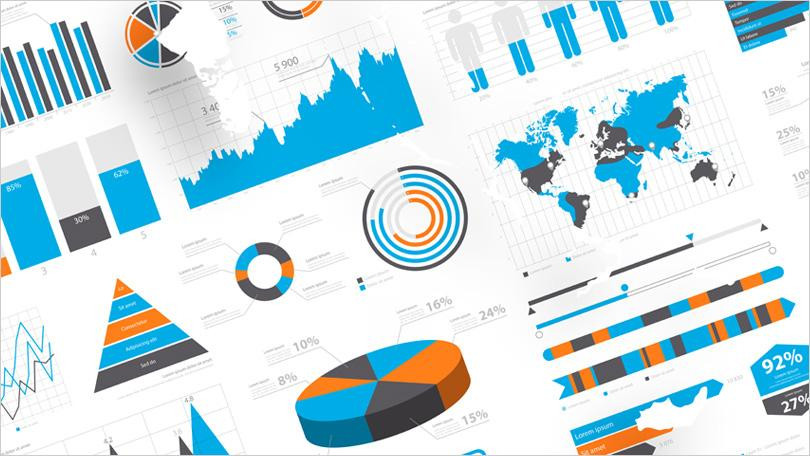
\includegraphics[scale=.30]{aula-2/figuras/matplot-dataviz-a.jpg}
  \end{figure}
\end{frame}
%

 